\documentclass[a4paper]{article}

\usepackage[english]{babel}
\usepackage[utf8]{inputenc}
\usepackage{amsmath}
\usepackage{graphicx}
\usepackage{subfigure}

\usepackage[colorinlistoftodos]{todonotes}
% 导入包
\usepackage{hyperref}
% 格式设置
\hypersetup{hidelinks,
	colorlinks=true,
	allcolors=black,
	pdfstartview=Fit,
	breaklinks=true}
	
\title{EDA234 Lab 1:  Lab Tutorial}

\author{Weihan Gao weihanga@chalmers.se} 

\date{\today}

\begin{document}
\sloppy
\maketitle


\section{First step}
\label{sec:introduction}
We implemented the second counter in three modules – Cntsecond\_forBolt.vhdl, digital\_show.vhdl and top.vhdl. Cntsecond module counts the 1Hz clk\_1s and generates the 2 numbers – cnt\_L and cnt\_H, ranging from 0 to 9 and 0 to 5. They will be shown on two digital segments through the digital\_show module at nearly 200Hz. Top module contains these two modules and has a process to divide the system clk frequency(100MHz) into the two clks we want.


The partner in the lab is Yuxiang Cao.

\begin{figure}[h]
\centering
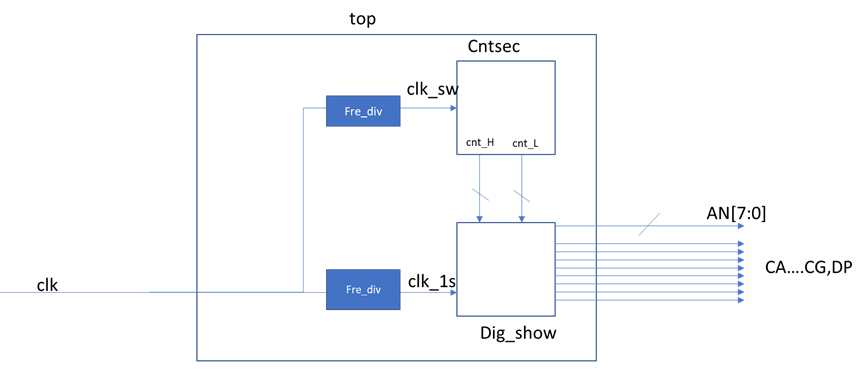
\includegraphics[width=1\textwidth]{1.png}
\caption{\label{fig:data}Simple block diagram.}
\end{figure}


\newpage

\section{Second step}
The registers we used are about 70 after initial implementation. And we first thought to reduce the use of sequential logic. So we put the case(for encoding) out of the rising\_edge in digital\_show.vhdl and the number of regs is down to 63.


\begin{figure}[h]
\centering
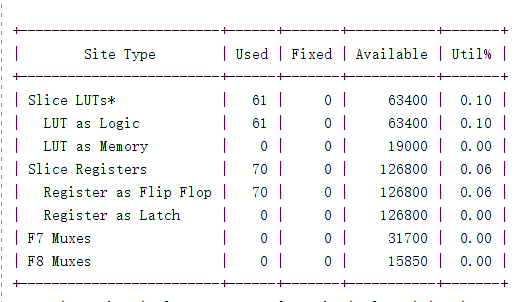
\includegraphics[width=0.6\textwidth]{2.png}
\caption{\label{fig:data}Initial number of regs.}
\end{figure}



\begin{figure}[h]
\centering
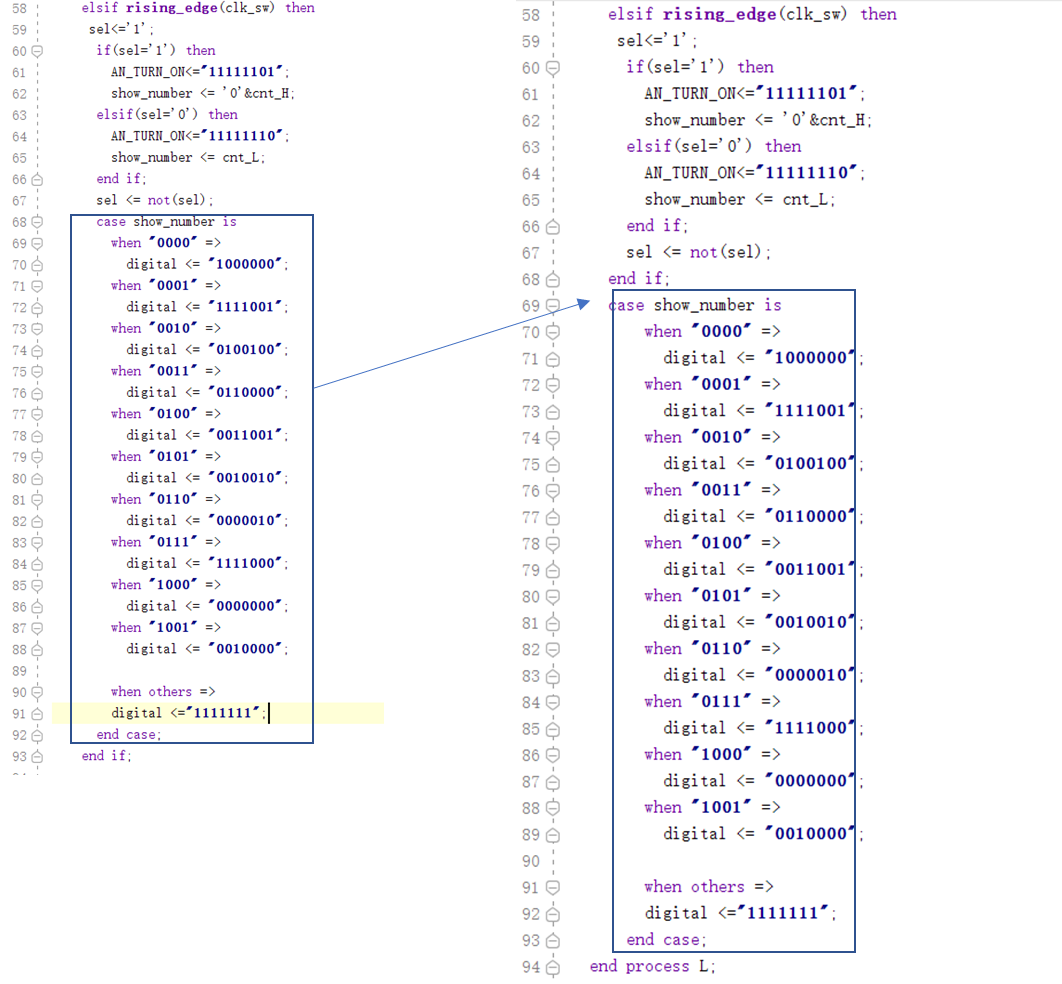
\includegraphics[width=0.8\textwidth]{3.png}
\caption{\label{fig:data}Put the case out of rising\_edge(clk\_sw).}
\end{figure}


\newpage

\begin{figure}[t]
\centering
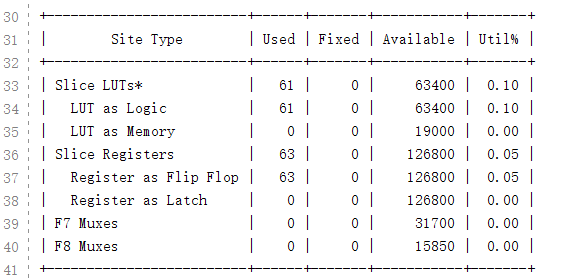
\includegraphics[width=0.8\textwidth]{4.png}
\caption{\label{fig:data}Number of regs after first modification.}
\end{figure}

\newpage

Then we found the biggest part of regs is those in LUT, which means two counters in fre\_div at top are over the limit. We could use only one counter to reach the requirement by containing the smaller counter in a bigger one. Finally, we used 43 regs and no latch.


\begin{figure}[h]
\centering
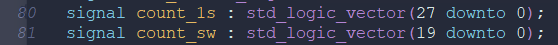
\includegraphics[width=1\textwidth]{5.png}
\caption{\label{fig:data}Two counters for freq\_div.}
\end{figure}



\begin{figure}[h]
\centering
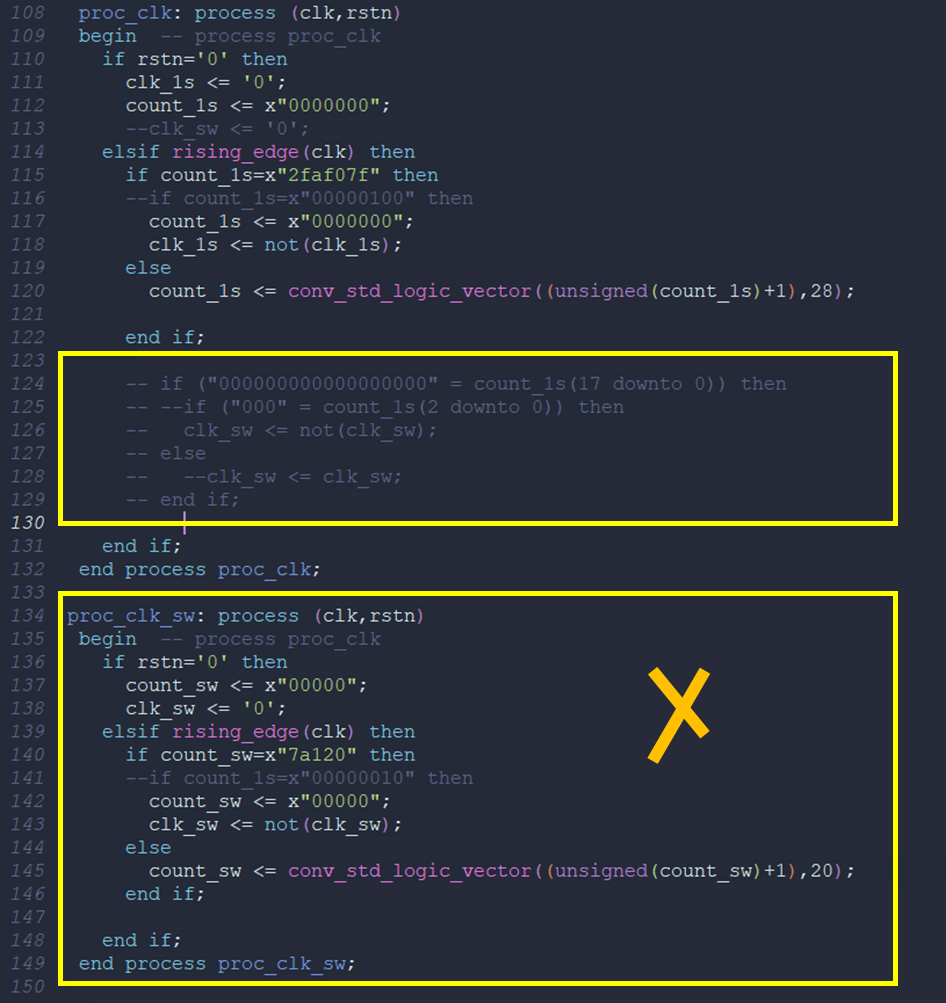
\includegraphics[width=1\textwidth]{6.png}
\caption{\label{fig:data}Delete the clk\_sw proc and put them in the clk\_1s proc. When the number is 2\^18, the clk\_sw flips.}
\end{figure}



\begin{figure}[h]
\centering
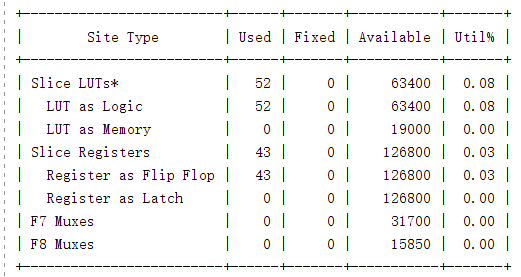
\includegraphics[width=1\textwidth]{7.png}
\caption{\label{fig:data}Final regs we used.}
\end{figure}





























\iffalse
\section{Experiment 1-2 pages}
\subsection{Fabrication}
Explain a step-by-step recipe for fabrication here. How long did you etch and why? What is an Ohmic contact?
\subsection{Experimental set-up}
Explain the experimental set-up here. Use a schematic picture (make it yourself in photoshop, paint, ...) to show how the components are connected. Briefly explain how a lock-in amplifier works.

\section{Results and interpretation 2-3 pages}
Show a graph of the longitudinal resistivity ($\rho_{xx}$) and Hall resistivity ($\rho_{xy}$) versus magnetic field, extracted from the raw data shown in figure \ref{fig:data}. You will have the link to the data in your absalon messages, if not e-mail Guen (guen@nbi.dk). Explain how you calculated these values, and refer to the theory.

\begin{figure}
\centering
\includegraphics[width=1\textwidth]{raw_data.png}
\caption{\label{fig:data}Raw (unprocessed) data. Replace this figure with the one you've made, that shows the resistivity.}
\end{figure}

\subsection{Classical regime}
Calculate the sheet electron density $n_{s}$ and electron mobility $\mu$ from the data in the low-field regime, and refer to the theory in section \ref{sec:theory}. Explain how you retrieved the values from the data (did you use a linear fit?).
Round values off to 1 or 2 significant digits: 8.1643 ~= 8.2. Also, 5e-6 is easier to read than 0.000005.

!OBS: This part is optional (only if you have time left).
Calculate the uncertainty as follows: \newline $u(f(x, y, z)) = \sqrt{(\frac{\delta f}{\delta{x}} u(x))^{2} + (\frac{\delta f}{\delta{y}} u(y))^{2} + (\frac{\delta f}{\delta{z}} u(z))^{2}}$, where $f$ is the calculated value ($n_{s}$ or $\mu$), $x, y, z$ are the variables taken from the measurement and $u(x)$ is the uncertainty in x (and so on).

\subsection{Quantum regime}
Calculate $n_{s}$ for the high-field regime.
Show a graph of the longitudinal conductivity ($\rho_{xx}$) and Hall conductivity($\rho_{xy}$) \textbf{in units of the resistance quantum} ($\frac{h}{e^{2}}$), depicting the integer filling factors for each plateau.
Show a graph of the plateau number versus its corresponding value of $1/B$. From this you can determine the slope, which you use to calculate the electron density.
Again, calculate the uncertainty for your obtained values.

\section{Discussion 1/2-1 page}
Discuss your results. Compare the two values of $n_{s}$ that you've found in the previous section. Compare your results with literature and comment on the difference. If you didn't know the value of the resistance quantum, would you be able to deduce it from your measurements? If yes/no, why?

\newpage
\section{Some LaTeX tips}
\label{sec:latex}
\subsection{How to Include Figures}

First you have to upload the image file (JPEG, PNG or PDF) from your computer to writeLaTeX using the upload link the project menu. Then use the includegraphics command to include it in your document. Use the figure environment and the caption command to add a number and a caption to your figure. See the code for Figure \ref{fig:frog} in this section for an example.

\begin{figure}
\centering
\includegraphics[width=0.3\textwidth]{frog.jpg}
\caption{\label{fig:frog}This frog was uploaded to writeLaTeX via the project menu.}
\end{figure}

\subsection{How to Make Tables}

Use the table and tabular commands for basic tables --- see Table~\ref{tab:widgets}, for example.

\begin{table}
\centering
\begin{tabular}{l|r}
Item & Quantity \\\hline
Widgets & 42 \\
Gadgets & 13
\end{tabular}
\caption{\label{tab:widgets}An example table.}
\end{table}

\subsection{How to Write Mathematics}

\LaTeX{} is great at typesetting mathematics. Let $X_1, X_2, \ldots, X_n$ be a sequence of independent and identically distributed random variables with $\text{E}[X_i] = \mu$ and $\text{Var}[X_i] = \sigma^2 < \infty$, and let

\begin{equation}
S_n = \frac{X_1 + X_2 + \cdots + X_n}{n}
      = \frac{1}{n}\sum_{i}^{n} X_i
\label{eq:sn}
\end{equation}

denote their mean. Then as $n$ approaches infinity, the random variables $\sqrt{n}(S_n - \mu)$ converge in distribution to a normal $\mathcal{N}(0, \sigma^2)$.

The equation \ref{eq:sn} is very nice.

\subsection{How to Make Sections and Subsections}

Use section and subsection commands to organize your document. \LaTeX{} handles all the formatting and numbering automatically. Use ref and label commands for cross-references.

\subsection{How to Make Lists}

You can make lists with automatic numbering \dots

\begin{enumerate}
\item Like this,
\item and like this.
\end{enumerate}
\dots or bullet points \dots
\begin{itemize}
\item Like this,
\item and like this.
\end{itemize}
\dots or with words and descriptions \dots
\begin{description}
\item[Word] Definition
\item[Concept] Explanation
\item[Idea] Text
\end{description}

We hope you find write\LaTeX\ useful, and please let us know if you have any feedback using the help menu above.

\begin{thebibliography}{9}
\bibitem{nano3}
  K. Grove-Rasmussen og Jesper Nygård,
  \emph{Kvantefænomener i Nanosystemer}.
  Niels Bohr Institute \& Nano-Science Center, Københavns Universitet

\end{thebibliography}
\fi



\end{document}